\RequirePackage[l2tabu, orthodox]{nag} % tells you of any bad LaTeX usage
                                       % must be first thing in class (with the exception of comments)

%% There is one option you should define; oneside or twoside
%% Use twoside for your viva docs (examiners hate long docs they need to carry around)
%% and oneside for the final thing you submit to the library.  Note that margins will
%% change accordingly

\documentclass[oneside]{um}  % custom University of Malta project/dissertation/thesis 


%% **************** (Your) Packages (Start) ******************

% \listfiles % uncomment this to know which packages you are using
              % the list of packages will be in the bottom of the .log file

%% Note that packges may already be loaded from the um (and memoir) classes.
%% Do not add your packages to the template, but rather add them here.
\usepackage{subfigure}
\usepackage{subcaption}
\usepackage{pythontex}
\usepackage{blindtext} %% for some dummy text, remove in your writeup

%% ***************** (Your) Packages (End) *******************


%% **************** (Your) Data (Start) ******************

\title{Constraints on VCG Model \\from GW Merger Events}  % use \\ here otherwise you get a justified title
                                                    % note capitalization of the title (only common 
                                                    % words in lower case)
%\tagline{Team Exouls}                     % tag line
\author{Astrophysics- B2}                           % your name
\authorID{123456M}                           % your University Identifier
\supervisor{Dr. Geetanjali Sethi}                             % your supervisor(s) name - no . in Dr
 
                                                    % simply comment out the above line if absent
\department{Astronomy and Astrophysics}                  % your department (e.g. Artifical Intelligence)
\faculty{Research Fellowship Program}                      % your faculty (e.g. ICT)
\degree{research fellowship}                      % the degree you are reading
                                                    % note the \ after the dot, so not to consider it a fullstop
\doctype{project report}                              % the type of document (fyp, dissertation, thesis)
\degreedate{\today}                        % when did you submit -- officially after your corrections !
%%\subjectcode{ICS5200}                               % the study unit-code (currently not used)

%% ***************** (Your) Data (End) *******************


%% ******** (Your) Document Settings (Start) *************

% You should have an images directory in every chapX subdirj
% NOTE:  Trailing / for subdirs is required.
\graphicspath{{./images/}{./chap1/images/}}   % Paths where to look for images, if defined "images" must always be there as it holds the images in-use by the template.

\makeindex

%% ********* (Your) Document Settings (End) **************

\begin{document}
\frontmatter 
    \maketitle       
    \begin{dedication}
{\large{To The Curious Kid In Everyone}}\\[4mm]
Never stop dreaming!
\end{dedication}

        % include a dedication.tex file
    \newgeometry{left=1.3cm,right=1.3cm, top=4cm}
\newcommand\blfootnote[1]{%
  \begingroup
  \renewcommand\thefootnote{}\footnote{#1}%
  \addtocounter{footnote}{-1}%
  \endgroup
}
\begin{teammates}
\vspace*{-3mm}{\textcolor{white}{Team}}
    \large{\begin{enumerate}
    \item {}$^\mathsection{}^\dagger$Name 1, Department, University
    \item {}$^\dagger$Name 2, Department, University
    \item {}$^\dagger{}^\mathsection$Name 3, Department, University
    \item {}$^\mathsection$Name 4, Department, University
    \item {}$^\mathsection$Name 5, Department, University
    \item {}$^\dagger$Name 6, Department, University
    \item {}$^\dagger$Name 7, Department, University
    \item {}$^\dagger{}^\mathsection$Name 8, Department, University
    \end{enumerate}}
\blfootnote{$\dagger \;\;$ Task 1 (example - Theoretical and Mathematical Analysis)}
\blfootnote{$\mathsection \;\;$ Task 2 (example - Data Collection and Analysis)}
\end{teammates}
\restoregeometry\if@openright\cleardoublepage\else\clearpage\fi
    \newgeometry{left=2.5cm,right=2.5cm, top=4cm}
\begin{acknowledgements}
\vspace*{-3mm}{\textcolor{white}{Abstract}}\\
We thank Dr. Geetanjali Sethi for accepting to be our supervisor
and for suggesting us this topic in which we have developed a deep interest for our internship. Our gratitude is not only limited to his scientific experience that guided us towards the research project, but also includes insightful and valuable discussions, we had during our internship duration. We also express our deepest gratitude to her for her patience, continuous support, and giving us the freedom to learn at our own pace. \\\\
Clearly, this project would not have been possible without the support of --------. \\\\

Lastly, I would like to thank SARSTEM for generously sponsoring the project \\\\

\end{acknowledgements}
\restoregeometry   % include an acknowledgements.tex file
    %% For tips on how to write a great abstract, have a look at
%%	-	https://www.cdc.gov/stdconference/2018/How-to-Write-an-Abstract_v4.pdf (presentation, start here)
%%	-	https://users.ece.cmu.edu/~koopman/essays/abstract.html
%%	-	https://search.proquest.com/docview/1417403858
%%  - 	https://www.sciencedirect.com/science/article/pii/S037837821830402X

\newgeometry{left=2.5cm,right=2.5cm, top=4cm}
\begin{abstract}
\vspace*{-3mm}{\textcolor{white}{Abstract}}\\
In this report, the parameters of the Variable Chaplygin Gas model, $\Omega_{m}$ and $n$, were constrained by finding the best fit between the observed value of the luminosity distance and distance modulus of Supernova events and Gravitational Wave Events at different redshifts to the theoretical values predicted by the Variable Chaplygin Gas model.
\end{abstract}
\restoregeometry\if@openright\cleardoublepage\else\clearpage\fi
    \newgeometry{left=3cm,right=3cm}
    \tableofcontents*\if@openright\cleardoublepage\else\clearpage\fi
    \listoffigures*\clearpage
    \listoftables*\clearpage
    %\lstlistoflistings*\clearpage
    %%% will only print what is used ... useful.
%% also acronyms are clickable, which is awesome

\chapter*{List of Abbreviations}
\markboth{List of Abbreviations}{List of Abbreviations}
               
\begin{acronym}\itemsep-20pt\parsep-20pt %% if you remove these spacing params this list becomes huge!
\item[BAO]  Baryon Acoustic Oscillations
\item[CG] Chaplygin Gas
\item[CBC] Compact Binary Coalescence
\item[CMBR] Cosmic Microwave Background Radiation
\item[FLRW] Friedmann–Lemaître–Robertson–Walker metric
\item[GRBs] Gamma-ray Bursts
\item[GR]   General Relativity 
\item[$ΛCDM$] Lambda cold dark matter
\item[OCG] Original Chaplygin Gas
\item[VCG] Variable Chaplygin Gas
\end{acronym}\clearpage\fi

%% Note: always use \input as you cannot nest \includes (amongst other things)
\pagestyle{umpage}
\mainmatter 
    \newgeometry{top=3.8cm,bottom=3.8cm,left=2.5cm,right=2.5cm}
    

% --------------------------------------------------------------


\chapter{Introduction}
\section{Motivation}
It is most often that the observations have the power to push the well established field to its most stringent tests. One such observation was of the supernovae type-Ia (SNe-Ia) which established that the universe is expanding. After SNe-Ia observation, there has been number of other observations which establishes that the expansion is accelerating such as Baryon Acoustic Oscillations (BAO), Cosmic Microwave Background Radiation(CMBR), Gamma-ray Bursts (GRBs). The observational results of SNe-Ia together with CMBR power spectrum show that our universe is mainly made up of two components: dark matter and dark energy. The dark matter contribute one-0third of the total energy density of the universe whereas dark energy contributes two-third of the total energy density of the universe.\\
In fact, it was in 1920s when Alexander Friedmann and Georges Lemaître independently provided first cosmological model which explains that the universe is expanding. There are many different cosmological models which explain the expanding universe. One such model which is most favourable is $\Lambda$CDM model (Lambda cold dark matter) where $\Lambda$ is the cosmological constant. This model is referred to as the standard model of Big Bang cosmology but it suffers from fine tuning problem. Hence, there are many cosmological models which remains active areas of research in cosmology today and they all involve trying to understand the nature of dark matter and dark energy. 
%------------------------------------------------
\section{Scope of this report in a nutshell}

The absolute scope of this project is to find the performance of a novel cosmological model with an new branch of astrophysics. The project will pave a way to test the credibility of General Relativity with the Cosmology as the terms like Redshift and Luminosity Distance of the Gravitational Wave Merger Events are determined from our knowledge on General Relativity. Meanwhile the performance of Variable Chaplygin Gas in both Supernovae Dataset and Gravitational Waves Merger Event Dataset and comparing the results obtained from them helps us to calibrate our current understanding on the universe.    
    \chapter{Variable Chaplygin Gas}
\label{sec:2}
\section{Overview}
In 1920s, Alexander Friedmann theorized that the Universe is expanding using Einstein field equations after Vesto Slipher identified redshift of many galaxies. This theory was proved by the observational evidences from Edwin Hubble. George Lemaitre provided the linear relation between the distance of the galaxy and the redshift observed in them due to expansion of the universe. 
In early 1990s, with the observations of type Ia Supernovae (SNeIa) by independent research groups Supernova Cosmology Project (SCP) and the High-Z Supernova Search, the expansion of the universe was found to be accelerated compared to the initial assumption of the linear expansion by George Lemaitre. By the Friedmann-Robertson-Walker metric of the Universe, the expansion is directly proportional to the amount of matter present in the Universe. With accelerated expansion, the universe needed additional presence of mass or energy to be explained with the current cosmological model. With no evidence on these additional matter from Electromagnetic Radiations, this additional energy termed as Dark Energy. 

Similarly in 1930s, Fritz Zwicky found it in the Coma cluster that mass of the galaxies has to be higher than the visible matter to validate the higher orbital speed of the periphery of the galaxies. He proposed a presence of electromagnetically "dark matter" causing such anomalous high speed of rotations. This was proved by observations of Vera Rubin and others in 1970s and the theory of Dark Matter came into consideration.  

The pressing need to explain such phenomenon resulted in theorizing models which clubbed in these exotic entities in them. The presence of these entities brought in the $\Lambda$CDM ($\Lambda$ Cold Dark Matter) Model where $\Lambda$ denotes the Dark Matter and Dark Energy being the dominant entities in the universe under this model. With new insights on the universe, like Inflation Epoch and also with problems like fine tuning problem, the model has to modified to a more conclusive models validating the observations. One such model is the Chaplygin Gas Model.
 
\section{Modified gravity and Cosmological models}
All different models can be categorized into two classes. One class of models try to modify the geometry part of the Einstein's equation i.e. Einstein tensor $G_{ij}$. These theories are known as modified gravity. These are generalizations of the general relativity (GR) where gravity action is modified from $ A_{g}=\frac{-1}{16 \pi k} \int R \sqrt{-g} d^{4} x$ to $ A_{mg}=\frac{-1}{16 \pi k} \int f(R) \sqrt{-g} d^{4} x$ where $f(R)$ is a function of Ricci scalar,$A_g$ is the action for GR, $A_{mg}$ is the action for modified gravity. One can also work in higher dimensions instead of four as a part of modifying gravity. The other class of models assumes universe is governed by general relativity but alter the matter component of the Einstein's equation i.e. Energy-Momentum tensor $T_{ij}$. Models in both classes explain the expanding universe. It is not possible to explain the accelerated universe if only normal matter is taken into consideration. Hence, exotic matter i.e. dark matter has to be added to the energy momentum tensor. Models based on this dark matter can be further divided into quintessence models where slowly evolving and spatially homogeneous scalar field or two coupled fields are considered and dark energy models including barotropic fluids. Quintessence models also suffer from fine tuning problem, therefore, possible alternative which we should look into is dark energy models like barotropic fluids.\\
%--------------------------------------------------------------------------------------------------------------------------------------
\subsection{Dark Energy vs Normal Matter}\label{sec2}
The dark energy in contrast to normal matter has the negative pressure.



\section{Chaplygin Gas Model}
Dark energy models including barotropic fluids have pressure as a function of energy density, $P=f(\rho)$, which determines the dynamics of the fluid. These models also contains classes with varying equation of state. One specific example of the barotropic fluid is Chaplygin gas (CG) whose equation of state is $P=-A/\rho$, where A is a positive constant. Chaplygin gas  model  correctly describes the effects  of  dark  energy  and  dark  matter,  and  is a alternate for our current standard model of cosmology. As described in the previous section dark energy models have negative pressure, CG model also has a negative pressure associated with it and the more generalized model of CG is described by the equation of the sate given as
\begin{equation}\label{ch}
    p=-\frac{A}{\rho ^\alpha}
\end{equation}
where p is the pressure, $\rho$ is the energy density, both in a comoving reference frame with $\rho>0$, A and $\alpha$ ($0<\alpha \leq 1$) are positive constants ($\alpha=1$ corresponds to CG). In FLRW metric, energy conservation equation is given by
\begin{equation}\label{conseq}
    \dot{\rho}_{i}+\frac{3 \dot{a}}{a}\left(p_{i}+\rho_{i}\right)=0
\end{equation}
This is the fluid equation which holds for radiation(r), Baryonic matter(b) and chaplygin gas(ch), i.e. $i={r,b,ch}$. In this report, we assume the universe is filled with CG-radiation-baryonic matter. Using \ref{ch} and \ref{conseq}, we can get the expression for the energy density of the CG given by 
\begin{equation}\label{CGdensity}
    \rho_{ch}=\left(A+\frac{B}{a^{3(1+\alpha)}}\right)^{\frac{1}{1+\alpha}}
\end{equation}
where B is the constant of integration and a is the scale factor. Hence, we got the equation of state and energy density of the CG model given by \ref{ch} and \ref{CGdensity} respectively. We can similarly find the  energy density for baryonic matter and radiation given their equation of state. \\
Equation of state for baryonic matter is $p=0$. Using energy conservation equation \ref{conseq} we can obtain the energy density of the baryonic matter given by 
\begin{equation}\label{bar}
    \rho_b=\rho_{b0} a^{-3}
\end{equation}
where $\rho_{b0}$ is the integration constant. Equation of state for the radiation is $p=\rho/3$. Radiation is the ideal fluid, hence, energy momentum tensor in curved spacetime can be written as $T^i_j=(p+\rho) U^i U_j - p g^i_j$. Taking trace of this equation we get $T^i_j= p+\rho -4p=\rho-3p$. Using equation of state we get the trace of the energy momentum tensor for the radiation to vanish. This vanishing of trace of $T_I_j$ is a common feature for theories which are conformally invariant. Anyways, repeating the same story which we did for CG and baryonic matter i.e using energy conservation equation \ref{conseq}, we can obtain the energy density of the radiation which is given by
\begin{equation}\label{rad}
    \rho_r=\rho_{r0}a^{-4}
\end{equation}
Total energy density can be written as the sum of the components \ref{CGdensity}, \ref{bar}, \ref{rad}, given by
\begin{equation}\label{tot}
    \rho_{total}(a)=\left(A+\frac{B}{a^{3(1+\alpha)}}\right)^{\frac{1}{1+\alpha}} + \rho_{b0} a^{-3} + \rho_{r0}a^{-4}
\end{equation}
The Friedmann equation gives the expansion rate of the Universe in terms of matter and radiation density,$\rho$, curvature,k, and the cosmological constant,$\Lambda$, as
\begin{equation}\label{freidmann}
    H^{2} \equiv\left(\frac{\dot{a}}{a}\right)^{2}=\frac{8 \pi G}{3} \rho-\frac{k}{a^{2}}+\frac{\Lambda}{3}
\end{equation}
where $H\equiv \frac{\dot a}{a}$ is the Hubble parameter. Assuming spatially flat universe, we get
\begin{equation}
    H^{2}=\frac{8 \pi G}{3} \rho
\end{equation}
Using total energy density expression \ref{tot}, Freidmann equation \ref{freidmann} reads as
\begin{equation}
    3 H^2= 8\pi G\left(A+\frac{B}{a^{3(1+\alpha)}}\right)^{\frac{1}{1+\alpha}} + \rho_{b0} a^{-3} + \rho_{r0}a^{-4}
\end{equation}
We can also make change of variables and use redshift, z, instead of using scale factor, a, which is not a physically measurable quantity. The relation between redshift and scale factor is given by
\begin{equation}\label{RDZ}
    1+z=\frac{a_0}{a}
\end{equation}
where $a_0$ is the scale factor at the present time which we normalize to 1. Freidmann's equation in terms of redshift can be written as
\begin{equation}\label{Freidredshift}
3 H^{2}(z)=\left\{\left[A+B(1+z)^{3(1+\alpha)}\right]^{\frac{1}{1+a}}+\left(\rho_{r0}\right)(1+z)^{4}+\left(\rho_{b0}\right)(1+z)^{3}\right\}
\end{equation}
\subsection{Evolution of Chaplygin Gas}
We can determine the evolution of the energy density of the CG during different epochs by analyzing equation \ref{CGdensity}. At early times, $a<<1$, \ref{CGdensity} can be written as 
\begin{equation}
    \rho_{ch}=\frac{B^{1/(1+\alpha)}}{a^3}
\end{equation}
Original CG energy density by using $\alpha=1$ can be written as
\begin{equation}
      \rho_{ch}=\frac{\sqrt{B}}{a^3}
\end{equation}
Therefore, at early times OCG corresponds to dust like matter(or dark matter). On the other hand, at late times we can similarly show that
\begin{equation}
    \rho_{ch}= -p = A^{1/(1+\alpha)} = Constant
\end{equation}
Following the discussion in \ref{sec2}, we can conclude that CG at late times corresponds to a cosmological constant. Thus leads to the observed accelerated expansion. Therefore, we can further conclude that CG evolves from the dust dominated epoch to cosmological constant in present times, and thus CG model can unify CDM and the $\Lambda$ model features. Therefore, the CG model is a good alternative to explain the accelerated expansion of the universe. However the CG model produces an exponential blowup of matter power spectrums that are inconsistent with observations. Due to this, a modification of the CG model is proposed called Variable Chaplygin Gas model.
\section{Variable Chaplygin Gas Model}
Equation of state of the Variable Chaplygin Gas (VCG) is given by
\begin{equation}\label{VCG}
    \rho_{ch}=\frac{A(a)}{p}
\end{equation}
where where p is the pressure, $\rho$ is the energy density, both in a comoving reference frame with $\rho>0$, $A(a) = A_0 a^{-n}$ is a positive function of the cosmological scale factor a. $A_0$ and n are constants. Using \ref{conseq}, we can find the energy density of VCG as
\begin{equation}\label{EDVCG}
    \rho_{c h}=\sqrt{\frac{6}{6-n} \frac{A_{0}}{a^{n}}+\frac{B}{a^{6}}}
\end{equation}
where B is the positive integration constant. For n=0, OGC behaviour is recovered. Assuming universe to be spatially flat, 2nd Freindmann equation can be written as 
\begin{equation}
    2\frac{\ddot a}{a} + H^2=-\frac{8 \pi G}{c^2} p
\end{equation}
The acceleration condition, $\ddot a$ can be written as
\begin{equation}
    (H^2 +\frac{8\pi G}{c^2}p)a<0
\end{equation} 
Using equation of state of VCG \ref{VCG} and energy density of VCG \ref{EDVCG}, we find the above acceleration condition is equivalent to 
\begin{equation}
    3 \frac{4-n}{6-n} a^{6-n} >\frac{B}{A_0}
\end{equation}
As both B and $A_0 $ are positive constants, hence $n<4$. At present time, a=$a_0 $= 1, hence, the present value of the energy density of VCG is given by
\begin{equation}
    \rho_{ch0}=\sqrt{\frac{6}{6-n} A_{0}+B}
\end{equation}
Defining the parameter, $\Omega_m$,
\begin{equation}
    \Omega_{m}=\frac{B}{6 A_{0} /(6-n)+B}
\end{equation}
the energy density becomes
\begin{equation}\label{VCGdensity}
    \rho_{ch}(a)=\rho_{c h 0}\left[\frac{\Omega_{m}}{a^{6}}+\frac{1-\Omega_{m}}{a^{n}}\right]^{1 / 2}
\end{equation}

Total energy density of the universe can be written as the sum of components \ref{VCGdensity}, \ref{bar}, \ref{rad}, given by
\begin{equation}\label{totVCG}
    \rho_{total}(a)=\left(\rho_{c h 0}\left[\frac{\Omega_{m}}{a^{6}}+\frac{1-\Omega_{m}}{a^{n}}\right]^{1 / 2}\right) + \rho_{b0} a^{-3} + \rho_{r0}a^{-4}
\end{equation}
Defining $\Omega_{r0} = \frac{8 \pi G\rho_{r0}}{3H_0 ^2}$ and $\Omega_{b0} = \frac{8 \pi G\rho_{b0}}{3H_0 ^2}$, $\Omega_{ch0} = \frac{8 \pi G\rho_{ch0}}{3H_0 ^2}$ as dimensionless density parameters. The density parameters for radiation and baryonic matter can be expressed as
\begin{equation}
    \Omega_{r}(z)=\left(\Omega_{r0}\right)(1+z)^{4}, \quad \Omega_{b}(z)=\left(\Omega_{b0}\right)(1+z)^{3}
\end{equation}The total density parameter for a universe where CG, baryonic matter and radiation dominate can be written as
\begin{equation}
    1=\Omega_{r}(z)+\Omega_{b}(z)+\Omega_{e h}(z)
\end{equation}
Using total energy density expression \ref{totVCG} and \ref{RDZ}, Freidmann equation \ref{freidmann} in terms of redshift reads as
\begin{equation}
    H^2=\Omega_{ch0} H_0^2 (1+z)^4 X^2(z)
\end{equation}
where
\begin{equation}\label{Imp}
    X^{2}(z)=\frac{\Omega_{r 0}}{1-\Omega_{r 0}-\Omega_{b 0}}+\frac{\Omega_{b 0} }{1-\Omega_{r 0}-\Omega_{\theta 0}(1+z)}+\frac{\left(\Omega_{m}(1+z)^6+(1-\Omega_{m})(1+z)^n\right)^{1 / 2}}{(1+z)^4}
\end{equation}
To test VCG model, the above equation \ref{Imp} is useful. There are two free paramters in the above equation $\Omega_m$ and n. We can use the distance modulus,$\mu$, for Supernovae Type IA data and gravitational waves from compact binary coalescence's (CBCs), and calculate the corresponding distance modulus for the CG model at corresponding redshifts.








%-----------------------------------------------------------------------------------------------------------------------------------------







\section{Bibliography Notes}
This whole chapter was greatly influenced by chapter 2 from \citep{bertibangalore} and \citep{carroll2019spacetime}.






    \chapter{Standard Candles and Standard Sirens}
\label{sec:4} 
\section{Overview}
In order to peek further into space, we need to make use of the global properties of galaxies, for small-scale distance measurement methods are rendered useless here. This is where standard candles come into the picture. Standard candles are fictitious objects of constant luminosity for which apparent magnitude is directly related to distance. Supernova is a high-energy phenomena that takes place at the end of stellar evolution. Even-though the discrete objects in the far away galaxies become faint and hard to resolve, a supernova explosion makes an exception.The consistent luminosity curve and relatively homogeneous properties of a type Ia supernova make it the perfect choice of standard candle for a cosmologist. 

Standard sirens are excellent distance measurement tools. The standardized amplitude gives us the idea of how far the source is. The gravitational waves from the Merger Events are ripples in the spacetime fabric which due to the nature of the medium it is traversed, doesn't lose it's energy with interaction with any gravitating object, be it baryonic matter or exotic matter like dark matter - dark energy. 

Testing the performance of Variable Chaplygin Gas Model in two different energy spectrum, the electromagnetic radiations (Standard Candles) and gravitational waves (Standard Sirens) which are originated from two different events is a solid way to test the ability of the model to mimic the nature of the Universe. 
   
\section{Type Ia Supernova data set and calibration}
The SCP (Supernova Cosmology Project) Union 2.1 dataset is compilation of 833 Type Ia Supernovae events collected and merged from 19 individual dataset. We have taken 580 events from the overall dataset, as these events are completely verified and could be trusted with higher level of confidence. The dataset is consist of data like redshift obtained from the event, distance modulus of the event and the potential error factor involved in estimation of the distance modulus.

The luminosity distance of the Supernovae event could be expressed as a function of redshift of the event pertaining to the Variable Chaplygin Gas Model. In a flat universe in which the parameter are constrained by the Variable Chaplygin Gas Model, the luminosity distance can be express as  
\begin{equation}\label{3 Luminosity distance equation}
    d_L(z,\textbf{p}) = c{(1+z)}{\int_{0}^{z}\frac{dz'}{H(z',\textbf{p})}}
\end{equation}
where z is the redshift, H is given by 
\begin{equation}\label{3 H term}
    H^{2} = \frac{8{\pi}G}{3}({\rho_{r0}{(1+z)}^{4}+\rho_{b0}{(1+z)}^{3}+\rho_{ch0}{[{\Omega_{m}{(1+z)}^{6}+{(1-\Omega_{m}}){(1+z)}^{n}}]}^{1/2}})
\end{equation}
where $\rho_{r0}$ and $\rho_{b0}$ are the current energy densities of radiation and baryons in the universe. $\rho_{ch0}$ is the energy density of Variable Chaplygin Gas entity consist of Dark Matter and Dark Energy. The \textbf{p} in the previous equation denotes all other parameters of the given cosmological model.   

\section{Overview about the GW Merger Events Dataset}
The Gravitational Merger events are obtained from the GWOSC (Gravitational Wave Open Science Center) which has the events obtained from detectors at LIGO Hanford, LIGO Livingston and LIGO Virgo. The data set consist of many confirmed events and potentially true events which are yet to be confirmed in it. The events are collected across all the three runs: O1 (from 12 September 2015 to 19 January 2016), O2 (from 30 November 2016 to 25 August 2017) and the O3 runs, O3a (from 1 April 2019 to 30 September 2019) and O3b (from 1 November 2019 to March 2020).

There were in total 53 confirmed events in the currently data set. All these confirmed events were taken to test the efficiency of the Variable Chaplygin Gas Model to predict the luminosity distance of the event from the redshift obtained from the gravitational merger events and compare with luminosity distance obtained from the merger event by analysis of the wave received at the detector.

\section{Luminosity Distance from Merger Events}
When a gravitational wave passes through the laser interferometer, it elongates the distance between the source and the reflector in the end in one arm and contracts the reflector length from the source in the other arm which is almost perpendicular to the elongated arm. This alternative elongation and contraction in the perpendicular arms, due to the quadrupole nature of the gravitational waves, causes path difference between the laser beams running between the arms and results in interference. The beams from perpendicular arms are made to interfere destructively in the standalone state but produce light by the interference induced by the passage of gravitational waves. The extent of elongation or contraction is determined by the amplitude of the gravitational wave passing the detector.

Since gravitational waves distort the geometrical length between the arms to cause interference, the amplitude of the laser beam from the interference pattern is directly related to the amplitude of the gravitational wave signal from the merger event. The gravitational waves weakly interact with matter, so the amplitude measured in the detector is an absolute quantity that one could measure from the merger events which provides insights about the events.

The amplitude of the wave/signal from the merger event is a function of linear separation between the binary, angular velocity of the system and also inversely proportional to the distance at which the event has occurred. This amplitude is a scale to quantify the energy emitted from the merger event as gravitational waves. Therefore we can express Luminosity of the merger event as a function of angular velocity, angular separation and distance. This luminosity is analogous to the luminosity described for stellar objects in electromagnetic counterparts.
\begin{equation}\label{AmplitudeGW}
    h = {\frac{G^{5/3}}{c^{4}}}\frac{{\mu}{a^{2}}{\omega^{2}}}{r}
\end{equation}
where, h is the Amplitude of the wave , $\mu$ is the reduced mass of the system = $\frac{{m_1}{m_2}}{m_1+m_2}$, $m_1$ and $m_2$ are the mass which are part of the binary system, a is separation between masses, r-distance between observer and $\omega$ - orbital velocity.

\begin{equation}\label{luminosity}
L = \frac{dE_{GW}}{dt} \approx \frac{G}{c^{5}}{h^{2}}{\omega^{2}} \approx \frac{G}{c^{5}}{\mu^{2}}{a^{4}}{\omega^{6}}
\end{equation} 
where, $\frac{dE_{GW}}{dt}$ is the rate of energy emitted by the binary event as gravitational waves.

Luminosity is a measure of energy emission from a given source. In case of binary merger events, the energy is transferred from the lost orbital energy of the binary system as the masses inspiral towards each other. So, the ratio between the frequency and the rate of change of frequency is proportional to the ratio between the separation of the mass in the system and the rate of change of this separation at successive orbits.

\begin{equation}\label{ratio frequency and amplitude}
	\frac{\omega}{\dot{\omega}} = \frac{-3}{2}{\frac{a}{\dot{a}}} = \frac{f}{\dot{f}}
\end{equation}
where, f = $\frac{\omega}{\pi}$ is the frequency of the signal and $\dot{f}$ = $\frac{\dot{\omega}}{\pi}$ is the rate of change in frequency

The ratio of frequency to the rate of change of frequency can be found from the waveform of the signal. The iconic chirp waveform of the gravitational wave from the detector helps us in obtaining the maximum amplitude, frequency and its ratio to the rate of change of frequency. From the above information, the luminosity distance (in Megaparsec (Mpc)) of a merger event can be found:
\begin{equation}\label{Luminosity distance}
		R = \frac{512}{h_{21}}{(\frac{0.01}{\tau})}{(\frac{100 Hz}{f_{GW}})}^{2}
\end{equation}

the $\tau$ is the subtle expression for the ratio of the frequency of the gravitational wave to the rate of change in the frequency as the separation between the masses of the binary system gets reduced as they inspiral towards each other  
\begin{equation}\label{tau}
        \tau = \frac{f_{GW}}{\dot{f_{GW}}}
\end{equation}
where, R - luminosity distance, $h_{21}$ - amplitude caused by the inspiral of mass 1 and mass 2 of the binary system.  
\section{Distance Modulus - Flat $\Lambda$CDM Model and VCG Model}
The distance modulus is a logarithmic scaling term used to describe the distance of an energy radiating entity in astronomy. The distance modulus $\mu$ can be expressed as the difference between the apparent magnitude ($m$) and the absolute magnitude ($M$). 

\subsection{Supernova Type Ia dataset}

The distance modulus that is provided in the SNe-Ia dataset is given by the $\Lambda$CDM Model for a given redshift as
\begin{equation}
    \mu_{obs} = {a}(t_{0})r{\left(1+z\right)}
\end{equation}
where a is the scale factor. The scale factor (a) in a flat universe can be expressed as $\frac{1}{(1+z)}$. $t_{0}$ is the Hubble Time which is $\frac{1}{H_0}$, where $H_0$ is the Hubble Parameter value in the current epoch. z is the redshift value of the entity under study. 

The r in Eq. (3.8) is the coordinate distance. In a flat $\Lambda$CDM model universe, the r is expressed as
\begin{equation}
    r = \int_{t}^{t_0}\frac{cdt}{a(t)} = \frac{c}{a_0H_0}\int_{0}^{z}\frac{dz'}{h(z')}
\end{equation}
The $a_0$ is the value of the scale factor in the observer's immediate surrounding. It is found to numerically equal to 1. The $h$ is Hubble parameter value for the region of space of the given redshift. The $h$ is expressed as 
\begin{equation}
    h(z) = [\left(1-\Omega_{total})(1+z)^{2}+\Omega_{m}(1+z)^{3}+\Omega_{\Lambda}(1+z)^{p}\right]^{1/2}
\end{equation}
in a flat universe, $\Omega_{total}$ = 1 and p is numerically equal to 1. So, the equation becomes
\begin{equation}
    h(z)={[\left\Omega_{m}(1+z)^{3}+\Omega_{\Lambda}\right]}^{1/2}
\end{equation}
so,
\begin{equation}
\mu_{obs} = \frac{1}{H_{0}^{2}(1+z)}\frac{c}{a_0}\int_{0}^{z}\frac{dz'}{[\left\Omega_{m}(1+z')^{3}+\Omega_{\Lambda}\right]^{1/2}}
\end{equation}
the reason why the redshift (z) inside the integral is dashed is to differentiate it with the redshift term outside the integration, and to denote that the denominator of the integral as a variable entity unlike the redshift term outside the integral.

The redshift of the given supernova event is used to calculate the distance modulus of the event and it is available in the SCP dataset.

With the Variable Chaplygin Gas Model, the distance modulus is given as
\begin{equation}
    \mu_{th} = 5\log{d_{L}(z)}-5\log{h}+42.38 = 5\log{d_{L}(z)}+5log\left(\frac{cH_{0}}{1Mpc}\right)+25
 \end{equation}
the $d_{L}$ is obtained from equation 3.1 

\subsection{Gravitational Wave Merger dataset}
The standard distance modulus of the merger event is calculated from the luminosity distance obtained by the signal of the merger event as described in section 3.4 as
\begin{equation}
    \mu_{obs} = 5\log{d_{L}}-5
\end{equation}
where $d_{L}$ is the distance modulus obtained from the wave analysis. 

The $\mu_{th}$ part is obtained from Equation 3.13, where the $d_{L}$ is a function of redshift given by the wave analysis of signals from merger events. The expression for $d_{L}$ is given at Equation 3.1.

The $\mu_{obs}$ is termed as observed distance modulus that is given in the database from standard cosmological model, the $\Lambda$CDM Model. The $\mu_{th}$ is the theoretical distance model, obtained from Variable Chaplygin Gas (VCG) Model.

\section{Bibliography Notes}
Section 3.4 was influenced from \citep{bertibangalore}, section 4.3 was influenced by  \citep{leaver1985analytic}, and section 4.4 was heavily influenced by \citep{gurbir}.

    
\chapter{Statistical Analysis}
\label{sec:3}
\section{Overview}
In order to find the right combination of the constrains $\Omega_{m}$ and $n$ for which the model provides best fit of the luminosity distance and the distance modulus, a $\chi^{2}$ test is conducted between the observed values in the dataset and the calculated values from the model. $\chi$-squared is a test to verify a hypothesis proposed to explain the distribution in a given dataset. The hypothesis or the equation that is devised to fit the distribution of the data-points from given parameters are generally termed as Null Hypothesis. These null hypothesis when tested with a $\chi^{2}$ test provides a numerical value which defines the goodness of the hypothesis. This numerical value should be equal to or be around the numerical value of the total number of data-points involved in the dataset. $\chi$-squared test provides a clear picture on the performance of the model.   


\section{$\chi^2$ Test}
The standard equation to determine the goodness value of the $\chi^{2}$ test for distance modulus is given by
\begin{equation}
    \chi^{2} = \sum_{i}\left[\frac{\mu^{i}_{th}-\mu^{i}_{obs}}{\sigma_{i}}\right]
\end{equation}
where $\mu_{th}$ is the distance modulus value obtained from the theoretical calculation of the cosmological model and $\mu_{obs}$ is the observed value of distance modulus in the dataset. $\sigma$ is the possible magnitude of error in the observed distance modulus given by the dataset. The $\left[\frac{\mu_{th}-\mu_{obs}}{\sigma}\right]$ is calculated for each data-point and is summed for the total dataset.

In order to make to attribute the performance of other non constrained factors like the Hubble Parameter $H_0$, the equation is modified as
\begin{equation}
    \chi^{2} = \sum_{i}\left[\frac{\mu^{i}_{th}-\mu^{i}_{obs}}{\sigma_{i}}\right]-\frac{C_1}{C_2}{\left(C_1+\frac{2}{5}\ln{10}\right)}-2{\ln{h}}
\end{equation}
The terms $C_1$ and $C_2$ are given by
\begin{equation}
    C_1 = \sum_{i}\frac{\mu^{i}_{th}-\mu^{i}_{obs}}{\sigma_i^{2}}
\end{equation}
\begin{equation}
    C_2 = \sum_{i}\frac{1}{\sigma_i^{2}}
\end{equation}
$h$ is the dimensionless Hubble Parameter = $\frac{H_0}{100 (km)(s^{-1})(Mpc^{-1})}$


\section{Bibliography Notes}
Section 3.2 is influenced from \citep{bertibangalore} and rest of the sections were influenced by \citep{RevModPhys.70.1545} and \citep{nollert1999quasinormal}.
    \chapter{Discussion \& Conclusions}

% --------------------------------------------------------------

\section{Discussion}
\subsection{Calibration with SNe-Ia Dataset}
Before analyzing the performance of Variable Chaplygin Gas Model with Gravitational Merger Event, it has to be calibrated with respect to the SCP Union Type Ia supernovae data to compare the results of the model generated to the previous published results on the model to provide credibility to the model performance on Merger events.
Variable Chaplygin Model has a provided a best fit to the SNe-Ia dataset for $\Omega_{m}$ = 0.15 and n = 0.79 with a $\chi^{2}$ goodness value of 566.296 for the distance modulus.
\begin{figure}[h]\centering
{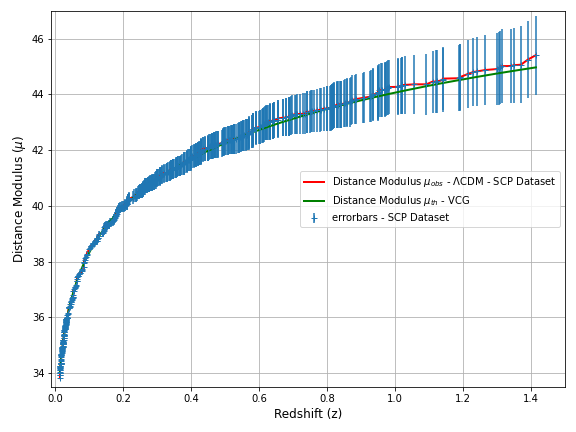
\includegraphics[width=13cm]{chap5/LCDM_DM_Redshift (1).png}
\caption{Performance of VCG Model to determine Distance Modulus (Green) with respect to the Distance Modulus from SCP Dataset (Red) against Redshift - $\Omega_{m}$=0.15, n = 0.79 and $H_{0}$=69.8}
\end{figure}

The performance VCG Model to determine luminosity distance is also included
\begin{figure}[h]\centering
{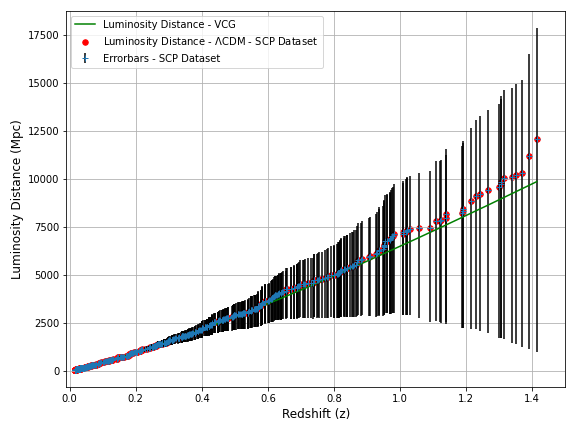
\includegraphics[width=13cm]{chap5/GoodLumi_Redshift.png}
\caption{Performance of VCG Model to determine Luminosity Distance (Green) with respect to the Luminosity Distance from $\Lambda$CDM Model (Red) against Redshift - $\Omega_{m}$=0.15, n = 0.79 and $H_{0}$=69.8}
\end{figure}

The graph depict the performance of the VCG devised against standard SCP Dataset. This provides credibility to the model has the predicted values of $\Omega_{m}$ and n closer to values from published papers: Guo & Zhong [$\Omega_{m}$=0.25, n=-2.9] and Sethi [$\Omega_{m}$=0.22, n=-2.8].
\subsection{Model performance on Gravitational Merger Events}
The Variable Chaplygin Gas Model, provided a best fit to the gravitational wave merger events obtained from GWOSC, for $\Omega_{m}$ = 0.17 and n = -8.7 with a $\chi^{2}$ goodness value of 0.388 for the distance modulus. 
\begin{figure}[h]\centering
{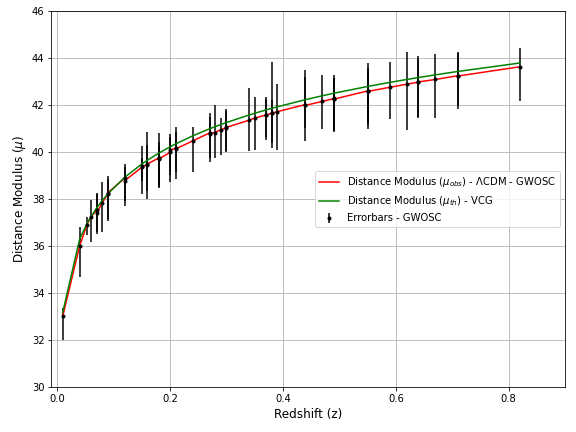
\includegraphics[width=13cm]{chap5/GW_DM.png}
\caption{Performance of VCG Model to determine Distance Modulus (Green) with respect to the Distance Modulus from $\Lambda$CDM Model (Red) against Redshift from GWOSC Dataset - $\Omega_{m}$=0.17, n = -8.7 and $H_{0}$=69.8}
\end{figure}

Similarily the perforance of VCG Model in determining Luminosity distance is given in the following plot 

\begin{figure}[h]\centering
{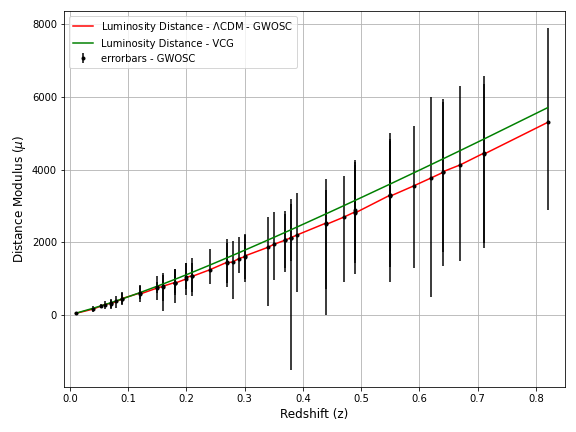
\includegraphics[width=13cm]{chap5/GW_Lumi_New.png}
\caption{Performance of VCG Model to determine Luminosity Distance (Green) with respect to the Luminosity Distance from $\Lambda$CDM Model (Red) against Redshift from GWOSC Dataset - $\Omega_{m}$=0.17, n = -8.7 and $H_{0}$=69.8}
\end{figure}

% --------------------------------------------------------------


    



% --------------------------------------------------------------

\chapter{Future Work}
\vspace*{-0.6cm}

% --------------------------------------------------------------

\section{Scope 1}
The GWOSC Dataset has added new confirmed events added from O3a and O3b runs. Including them into the dataset would be beneficial to constrain the cosmological parameters $\Omega_{m}$ and $n$ with tighter bounds.


% --------------------------------------------------------------

\section{Scope 2}
A contour plot to determine the validity of $\chi^{2}$ goodness value will be plotted. This provides more credible proof about the modified $\chi^{2}$ test that has been implemented for VCG Model. 




% --------------------------------------------------------------





% --------------------------------------------------------------
    \restoregeometry
    \newgeometry{top=3.8cm,bottom=3.8cm,left=2.2cm,right=2.2cm}
    \appendix
        \chapter{Appendix A}{\label{app:A}}
\vspace*{-0.7cm}

     % these are just test names as I didn't know what you'd want
        \chapter{Appendix B}
\vspace*{-1cm}
\lstinputlisting[style=Matlab-editor, caption={Code}]{programs/program.m}
    
        \chapter{Appendix C}
\vspace*{-1cm}
\lstinputlisting[style=Matlab-editor, caption={Code}]{programs/program.m} 
    
    
{\backmatter
    % Bibliography
    \if@openright\cleardoublepage\else\clearpage\fi
    \bibliographystyle{um-plainnat} %% specific plainnat does not show url for articles
    {\footnotesize\bibliography{background_and_lit_overview_biblio.bib}}
	\printindex
}\restoregeometry

\end{document}

%%% The End %%%